%\documentclass[letterpaper, 10 pt, conference]{ieeeconf}
%\usepackage{filecontents,lipsum}
%\usepackage[noadjust]{cite}
%%\begin{filecontents*}{references.bib}
%%@article{Khoe:1994:CML:2288694.2294265,
%%    author = {Khoe, G. -D.},
%%    title = {Coherent multicarrier lightwave technology for flexible capacity networks},
%%    journal = {Comm. Mag.},
%%    issue_date = {March 1994},
%%    volume = {32},
%%    number = {3},
%%    month = mar,
%%    year = {1994},
%%    issn = {0163-6804},
%%    pages = {22--33},
%%    numpages = {12},
%%    url = {http://dx.doi.org/10.1109/35.267438},
%%    doi = {10.1109/35.267438},
%%    acmid = {2294265},
%%    publisher = {IEEE Press},
%%    address = {Piscataway, NJ, USA},
%%}
%%\end{filecontents*}
%\title{This document}
%\author{This author}

%%%%%%%%%%%%%%%%%%%%%%%%%%%%%%%%%%%%%%%%%%%%%%%%%%%%%%%%%%%%%%%%%%%%%%%%%%%%%%%%
%2345678901234567890123456789012345678901234567890123456789012345678901234567890
%        1         2         3         4         5         6         7         8

\documentclass[letterpaper, 10 pt, conference]{ieeeconf}  % Comment this line out if you need a4paper

%\documentclass[a4paper, 10pt, conference]{ieeeconf}      % Use this line for a4 paper

\IEEEoverridecommandlockouts                              % This command is only needed if 
                                                          % you want to use the \thanks command

\overrideIEEEmargins                                      % Needed to meet printer requirements.

% See the \addtolength command later in the file to balance the column lengths
% on the last page of the document

% The following packages can be found on http:\\www.ctan.org
%\usepackage{graphics} % for pdf, bitmapped graphics files
%\usepackage{epsfig} % for postscript graphics files
%\usepackage{mathptmx} % assumes new font selection scheme installed
%\usepackage{times} % assumes new font selection scheme installed
%\usepackage{amsmath} % assumes amsmath package installed
%\usepackage{amssymb}  % assumes amsmath package installed
%\usepackage{filecontents,lipsum}
%\usepackage[noadjust]{cite}
%\usepackage{bm}
%\usepackage{tikz}
%\usepackage{graphicx}
%\usepackage{caption}
%\usepackage{subcaption}
%\usepackage{multicol}
%\usepackage{url}
%\usepackage{geometry}
%\usepackage{mathtools}
%\usepackage[utf8]{inputenc}
%\usepackage[english]{babel}
%\usepackage{algorithm}
%\usepackage[]{algpseudocode}


\usepackage{afterpage}
\usepackage{algorithm}
\usepackage[]{algpseudocode}
\usepackage{amsmath}
\usepackage{amssymb}  % assumes amsmath package installed
\usepackage{arydshln}
\usepackage[english]{babel}
\usepackage{bm}
\usepackage{caption}
\usepackage[T1]{fontenc}
\usepackage[]{graphicx}
\graphicspath{ {./fig/} }

\usepackage[utf8]{inputenc}
\usepackage{multicol}
\usepackage[T1]{xcolor}
\usepackage{soul}
\usepackage{subfig}
\usepackage{tikz}
\usepackage{url}
\usepackage[backend=biber,style=ieee,sorting=none]{biblatex}
\addbibresource{bib/references.bib}

\newcommand\blankpage{%
    \null
    \thispagestyle{empty}%
    \addtocounter{page}{-1}%
    \newpage}



\newcommand*{\important}[1]{\textcolor{red}{\danger~\textbf{IMPORTANT:~}} \textcolor{red}{#1}}

\newcommand*{\pending}[1]{\textcolor{blue}{$\bigstar$~\textbf{PENDING~#1}}}

\newcommand\mybox[2][]{\tikz[overlay]\node[fill=blue!100,inner sep=4pt, anchor=text, rectangle, rounded corners=1mm,#1] {#2};\phantom{#2}}

\newcommand{\TODO}{\mybox[fill=yellow]{\textcolor{blue}{\Large \textbf{TODO}}}}
\newcommand\myhl[1]{\textcolor{red}{#1}}


\newtheorem{prop}{Proposition}

\title{\LARGE \bf
Dynamic sensorimotor graphs
}


\author{Some Guy, Random Stranger and Anonymous Dude}

\begin{document}

\maketitle

\begin{abstract}
Regularities present in the sensorimotor signals of a robotic agent can reflect its embodiment, as well as the associations resulting from the active control policy. In this work, we analyze the functional connectivity of the sensorimotor signals based on pairwise mutual information. As the robot performs exploratory motions based on motor babbling we capture and study the time-varying changes in the relationships. We provide analysis of the instantaneous and average sharing of information and extrapolate the meaning in relation to the physical properties of the robot's body. Results from a simulated planar system validate the use of mutual information as a tool not only for the analysis of the relationships between the sensorimotor signals but also to drive exploratory motions.
\TODO
\end{abstract}
% =============================================================================
%                                                                             |
%                                                                             |
% ------------------------------- SECTION ------------------------------------|
%                                                                             |
%                                                                             |
% =============================================================================
\section{Introduction}\label{sec:intro}
\TODO
\begin{figure}[!ht]
	\centering
	\includegraphics[width=0.9\columnwidth]{general_overview.png}
	\caption{General overview.}
	\label{fig:general_overview}
\end{figure}

\subsection{Background}
This work explores the sensorimotor structure of an embodied agent. The underlying premise is that regularities among the robot's sensorimotor signals are a product of the robot’s embodiment. These regularities, known as \emph{sensorimotor contingencies} (SMC) \cite{Jacquey2019Sensorimotorcontingenciesas}, can be identified by studying the relationships between the signals from its sensory apparatus (for both perception and actuation). Information-theoretic metrics are considered to study the relationships in the sensorimotor system. Some examples of previous works that have used information theory in this context include  \cite{Schmidt2013Bootstrappingperceptionusing,Lungarella2006Mappinginformationflow,Polani2009Modelsinformationprocessing,Bossomaier2016introductiontransferentropy,Olsson2006unknownsensorsactuators}. Although the literature about sensorimotor representations is extensive \cite{Nguyen2021Sensorimotorrepresentationlearning}, this proposal considers that the representation of SMCs as \emph{dynamic} graphs and their corresponding analysis aided by concepts from graph theory could provide further understanding about their formation and evolution. To achieve such a representation, methods from \emph{network topology inference} (NTI)\cite{Dong2019Learninggraphsdata} are regarded to study the relationships among the different constituent elements of the graph.

Dynamical functional connectivity (DFC) has has mainly being used to study functional networks in the brain. For instance, in \cite{Christiaen2020Dynamicfunctionalconnectivity}, it was used to show states of lower functional connectivity during onsets of epilepsy.

The work in \cite{Zhou2020Earlychildhooddevelopmental} used NNMF on EEG signals to to identify potentially abnormal connectivity patterns in brains affected by illness.

\subsubsection{Tactile exploration}

\begin{itemize}
	\item The work by \cite{Gama2021Goaldirectedtactile} discussed the usage of intrinsic motivation and goal-babbling for learning self-touch on a simulated humanoid robot with artificial sensitive skin.
	\item Self-touch for calibration was used in \cite{Roncone2014Automatickinematicchain} letting the robot close the kinematic chain by touching its own body.
	\item \cite{Marcel2022Learningreachown} uses a multimodal variational autoencoder in a denoising framework to learn latent representation of self-touch that allows the agent to internally reconstruct self-reaching configurations. \myhl{The paper contributes to the sensorimotor contingency theory by providing a computational model that supports the hypothesis that the representation of self-touch can be learned simply through self-exploration.}
\end{itemize}








\subsubsection{Somatosensory relationships as graphs}
%---

	\textbf{How can information and graph theory be leveraged to devise a graphical representation of the SMCs in the somatosensory signals of a robot?}~\label{q4}

%---
As mentioned in \cite{Jacquey2019Sensorimotorcontingenciesas}, the connections between sensorimotor regularities and body knowledge are not well understood. To contribute to this understanding, this proposal parts from the knowledge of the number and modality of the robot's somatosensory signals (touch and proprioception) to%known, and metrics from information theory will be considered to evaluate the strength of the (possibly nonlinear) connections between pairs of sensor signals. Moreover, tools from graph theory will be used to define a sparse graph representing the most important connections. In short:
\begin{itemize}
	\item use information-theoretic metrics, such as mutual information, predictive information, and/or transfer entropy, to explore the functional connectivity among sensorimotor signals and
	\item leverage graph theoretical concepts to identify and study the most important sensorimotor connections.
\end{itemize}
% ---
As the statistical properties of the signals and their relationships may vary depending on the motion policy driving the robot or the task being executed by it, it is essential that the estimated graph shows plasticity to reflect these effects (see Fig.~\ref{fig:time_varying_network}). Therefore, unlike conventional NTI, methods that enable the estimated graph to change and adapt dynamically will be explored.
%---
%\begin{figure*}[htp!]
%	\centering	
%	\hspace*{\fill}
%	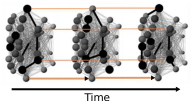
\includegraphics[width= 0.7\textwidth]{fig/time_varying_network.pdf}
%	\hspace*{\fill}
%	\caption[] {\label{fig:time_varying_network} Dynamic graph topology.}
%\end{figure*}
%---

% ---------------------------------------------------------------------------------------------------
% ---------------------------------------------------------------------------------------------------
%\subsubsection{Automatic generation of exploration trajectories}
%% ---
%\begin{shaded}
%	\question{How can exploratory motions be defined to result in informative data samples that expedite the learning of SMCs?}
%\end{shaded}
%% ---
%As the amount of data required to infer the sensorimotor graph poses a challenge, the robot needs to mindfully generate and adapt its body motions on-the-fly to collect relevant sets of data points. This proposal ponders the use of intrinsic motivation \cite{Oudeyer2007WhatisIntrinsic} to generate such motions. To define online exploration trajectories:
%%---
%\begin{itemize}
%	\item Metrics based on information theory, such as entropy, predictive information, and empowerment will be used to incite exploratory behavior.
%	\item Central Pattern Generators and chaotic systems will be contemplated as alternatives to generate cyclic and chaotic joint motions.
%	%	\item Methods to ensure the safety of the generated trajectories will be discussed.
%\end{itemize}

% SUBSECTION ==================================================================
\subsection{Related works}

Refer to Mannella, Gama, Marcel, Kanazawa, Husbands, Hoffmann (puppy).

% SUBSECTION ==================================================================
\subsection{Contributions}
With the goal of finding as much information as possible about body properties, we present an analysis based on the dynamic relationships existing among the sensorimotor signals of a embodied agent. In the analysis we show how the state of information sharing in the system is related to the motion of the robot and the tactile events that stem from its movement. By using non-negative matrix factorization we identified different information sharing states and classify them according to their information content. In a case study we demonstrate how after a motor babbling phase, by only focusing on the mutual information and without having knowledge about the morphology of the robot, an excitation trajectory for both the robot arms can be devised that avoids self contact. A comparison of this trajectory against conventional trajectory design methods is presented.

% =============================================================================
%                                                                             |
%                                                                             |
% ------------------------------- SECTION ------------------------------------|
%                                                                             |
%                                                                             |
% =============================================================================
\section{The embodied agent}


\subsection{Robot and measurements models}
% ---
%\begin{figure}[!t]
%	\begin{center}
%		\includegraphics[width=0.7\textwidth]{fig/planar_dual_arm.pdf}
%	\end{center}
%	\caption{\label{fig:planar_dual_arm} The planar dual arm.
%	}
%\end{figure}
% ---
This work takes as reference the robot model used in \cite{Mannella2018Knowyourbody,Marcel2022Learningreachown}, consisting of a simple six degrees-of-freedom planar dual arm system with three links per arm and a fixed torso, see Fig.~\ref{fig:extended_dual_arm_robot}. The robot is equipped with a set of tactile sensors distributed along the robot's body. They are modeled based on population coding \cite{Panzeri2010PopulationCoding} represented as Gaussian receptive fields (see Fig.~\ref{fig:population_coding}), with the means of the receptive fields randomly located along the robot's one-dimensional body. We modified the tactile sensors were modified to account for the strength of touch. Essentially, the previously distance-based activation of the Gaussian receptive fields in now scaled by the contact force. Furthermore, the dynamics of the model were instantiated by assigning inertial properties to the robot's composing bodies. Finally, we implemented the biology-inspired actuation model presented in \cite{Ekeberg1993combinedneuronalmechanical,Wadden1998neuromechanicalmodel, Shim2012Chaoticexplorationlearning}, where each joint is driven by antagonistic muscles (modeled as springs) whose pulling force is linearly controlled by the signal of a corresponding motor neuron $\sigma$. The generated joint torque, expressed as
% ---
\begin{equation}\label{eq:antagonistic_torque}
	\tau = \alpha \left(\sigma_{fx} - \sigma_{ex}\right)  + \beta \left(\sigma_{fx} + \sigma_{ex} + \gamma \right) q + \delta \dot{q},
\end{equation}
% ---
results from the difference between the flexion $ \sigma_{fx} $ and  extension $\sigma_{ex}$ activation signals which create the pulling forces $ f_{fx}$ and $f_{ex} $. The parameters are:
\begin{itemize}
	\item $\alpha$: muscle force gain
	\item $\beta$: stiffness gain
	\item $\gamma$: tonic stiffness	
	\item $\delta$: damping coefficient
\end{itemize}
%The model \eqref{eq:antagonistic_torque} also determines the joint stiffness via the term $\sigma_{fx} + \sigma_{ex}$. It is worth mentioning that the measurements corresponding to the pulling forces are also represented via population coding.

Similar to the tactile sensors, the robot's proprioceptive measurements are encoded using receptive fields. Originally, this model was meant to capture static relationships between joint configurations and touch/no-touch events. Therefore, the somatosensory measurements in the extended model consist of touch signals (scaled by the touch force) and proprioception that that encompasses joint position, velocity and effort.
%---
%\begin{figure*}[htp!]
%	\centering	
%	\hspace*{\fill}
%	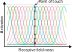
\includegraphics[width= 0.6\textwidth]{fig/receptive_fields.pdf}
%	\hspace*{\fill}
%	\caption[] {\label{fig:receptive_fields} The Gaussian receptive fields used in population coding.}
%\end{figure*}
%---

%The robot model in this work is based on the planar dual arm system with six degrees of freedom (DoF) used previously in \cite{Mannella2018Knowyourbody, Marcel2022Learningreachown}. The robot is equipped with a set of tactile sensors modeled as Gaussian receptive fields distributed along the robot's body. Motion of the robot was originally based on reference joint angle commands. We, however, have extended the model to instantiate its dynamics by assigning inertial properties to the robot's composing bodies. Furthermore, we changed the actuation mechanism inspired by simple muscle-inspired antagonistic joint model used in \cite{Shim2012Chaoticexplorationlearning}, where the muscle activation controls spring stiffness. The extended model is depicted on Fig.~\ref{fig:extended_dual_arm_robot}.
% ---
\begin{figure}[!t]
	\begin{center}
		\hspace*{\fill}
		\includegraphics[width=0.99\columnwidth]{extended_dual_arm_robot.pdf}
		\hspace*{\fill}
	\end{center}
	\caption{\label{fig:extended_dual_arm_robot} The planar dual arm robot.}
\end{figure}
% ---


% ---
\begin{figure}[!t]
	\begin{center}
		\hspace*{\fill}
		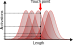
\includegraphics[width=0.99\columnwidth]{pop_coding_sketch.pdf}
		\hspace*{\fill}
	\end{center}
	\caption{\label{fig:population_coding} The receptive fields used in population coding.}
\end{figure}
% ---
% =============================================================================
%                                                                             |
%                                                                             |
% ------------------------------- SECTION ------------------------------------|
%                                                                             |
%                                                                             |
% =============================================================================
\section{The sensorimotor dynamic functional connectivity}

% Subsection ==================================================================
\subsection{Functional connectivity}
%Finding and graphically representing the relationships among the constituent elements of a system is known as \emph{network topology inference} (NTI) \cite{Dong2019Learninggraphsdata}. By learning the topology of a network (also known as a graph), it is possible to reveal a structure that aids in the analysis of the interaction among the entities. When relying only on measurement signals to estimate the network topology, approaches based on physically-motivated and statistical models are typically used\cite{Dong2019Learninggraphsdata}. In particular, the latter entails methods based on correlation, probabilistic graphical models, entropy, mutual information, and transfer entropy. Recently, other methods for NTI have been provided within the framework of Graph Signal Processing (GSP) \cite{Stankovic2019Introductiongraphsignal,Dong2019Learninggraphsdata,Mateos2019ConnectingdotsIdentifying}. Exemplary works showing the representation and analysis possibilities brought about by NTI include \cite{Zhang2017Networkbasedmachine,Karwowski2019Applicationgraphtheory,Sporns2018Graphtheorymethods}. 

\emph{Functional connectivity} (FC) is a method for network topology inference that characterizes the dependencies of the observed signals from a system based on their probability distributions\cite{Friston2011Functionaleffectiveconnectivity}. It can be subdivided into undirected and directed; the latter being related to the analysis of statistical causation from the data \cite{Bastos2016tutorialreviewfunctional}. By studying the FC  it is possible to reveal a structure that aids in the analysis of the interaction among the entities.

Based on the connection between embodiment and information structure \cite{Pfeifer2007Selforganizationembodiment}, our hypothesis is that properties of the sensorimotor interactions can be made apparent by studying the FC among the somatosensory signals $ \bm{x}(t) $. From the various metrics that have been proposed to evaluate such relationships, we in particular leverage those based on information theory \cite{Bonsignorio2020EntropyBasedMetrics,Bonsignorio2013Quantifyingevolutionaryself}, as their \emph{model-free} nature can capture linear and nonlinear relationships between signals. Particularly, we use the \emph{mutual information} (MI), a quantity that has been applied in different contexts to quantify the relationships between variables \cite{Steuer2002mutualinformationdetecting}. The MI between two signals $ I\left(X,Y\right) $ can be interpreted as the amount by which a random signal $ Y $ reduces the uncertainty about a random signal $ X $ \cite{Cover1999Elementsinformationtheory}. It is a symmetric measure of the information sharing by both signals and is computed as:
% ---
\begin{equation}\label{eq:mutual_information}
	I\left(X;Y\right) =I\left(Y;X\right) = H(X) + H(Y) - H(X,Y)
\end{equation}
% ---
with the Shannon's entropy of a variable $X$ defined by 
% ---
\begin{equation}\label{eq:entropy}
	H(X) = -\sum_{i=1}^{n}p(x_i)\text{log}_2\left(p\left(x_i\right)\right)
\end{equation}
% ---
and the joint entropy between $ X $ and $ Y $ expressed as
% ---
\begin{equation}\label{eq:joint_entropy}
	H(X,Y) = -\sum_{i=1}^{n}\sum_{j=1}^{n} p(x_i,y_j)\text{log}_2\big(p\left(x_i,y_j\right)\big).
\end{equation}
% ---
By extension, the mutual information matrix $ \hat{\bm{W}}_{MI} \in \mathbb{R}^{m \times m}$\footnote{We use the \emph{hat} notation to emphasize that this matrix is an estimate and there is no actual ground truth.} can be constructed by computing the pairwise MI between the $\left\lbrace x_i\right\rbrace^m_{i=1}$ somatosensory signals. Its $(i,j)$ entries are given by
% ---
\begin{equation}\label{eq:adjacency_mi}
	(\hat{\bm{W}}_{MI})_{i,j} = I(x_i,x_j).
\end{equation}
% ---
In practice, computing \eqref{eq:adjacency_mi}  for a pair $\left({x}_i(t),{x}_j(t)\right)$ of time series from the data matrix $\bm{X}$, centering their samples (to zero mean and unit standard deviation) and using either binning, kernel, or nearest neighbor methods \cite{WaltersWilliams2009Estimationmutualinformation} to compute their mutual information. 

%Yet, such a process can be memory- and computation-demanding when the length $n$ of each of the time series is large or when streaming signals are considered. \myhl{Therefore, to enable the online computation of the $m\left(m-1\right)/2$ pairwise MI values, every $N_{\mathbfcal{X}}$ points we extract a mini batch $\mathbfcal{X}$ from the replay buffer $\mathbfcal{B}$ and compute its corresponding MI matrix $\bm{W}^\mathbfcal{X}_{MI}$. Then, the overall MI matrix estimate $\hat{\bm{W}}_{MI}$ for the time series is the cumulative average over the previously computed matrices $\bm{W}^\mathbfcal{X}_{MI}$. To monitor its convergence we observe the total information content in the matrix, defined as
%	% ---
%	\begin{equation}\label{eq:total_information}
%		T_{MI} =  \frac{1}{2}\text{tr}\left(\hat{\bm{D}}_{MI}\right),
%	\end{equation}
%	% ---	
%	where $\hat{\bm{D}}_{MI}$ is the associated degree matrix. After the change in $T_{MI}$ falls below a threshold value $\epsilon$, i.e. 
%	$\Delta T_{MI}<\epsilon$, $\hat{\bm{W}}_{MI}$ exhibits minimal changes in its structure. In Sec.~\ref{sec:topology_convergence} we provide examples of the convergence of this term for the robot manipulator, hexapod, and humanoid cases.}

In this work, for the computation of $\hat{\bm{W}}_{MI}  $ we use the the open-source MATLAB package \emph{Mutual information computation}\cite{PengMutualInformationcomputation}.

% Subsection ==================================================================
\subsection{Dynamic functional connectivity}
When analizing FC it might be interesting to look not only at the aggregated effect of a complete dataset of recordings but also at the instantaneous changes that occur in the relationships. Indeed, the relationships between sensorimotor signals might change rapidly depending on the motion policy. To capture these time-varying functional connectivity with mutual information, the most common approach involves the usage of a sliding time window \cite{Preti2017dynamicfunctionalconnectome}. In particular, tactile events might have a short time scale, the nutual information was computed for a time window of length $T$, that is to say $x_i(t, t-1,\ldots, t-T)$, we called this term the \emph{instantaneous mutual information}.

\TODO


% ---
\begin{figure}[!th]
	\begin{center}
		\hspace*{\fill}
		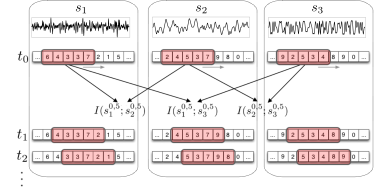
\includegraphics[width=0.99\columnwidth]{mi_sliding_window.png}
		\hspace*{\fill}
	\end{center}
	\caption{\label{fig:mi_sliding_window} Sliding window strategy to compute the instantaneous mutual information.}
\end{figure}
% ---

\begin{figure}[!th]
	\centering
	\includegraphics[width=0.9\columnwidth]{fig/nnmf.png}
	\caption{Decomposition of the mutual information data matrix using non negative matrix factorization.}
	\label{fig:nnmf}
\end{figure}

%\textbf{Rephrase:} \textit{To extract information from these connectivity graphs, the NMF \cite{Fu2019Nonnegativematrixfactorization} technique was used. NMF is an unsupervised machine learning algorithm that can be used to decompose an input matrix A into two components: a matrix W of bases, or subgraphs, and a matrix H of their corresponding contributions to the input matrix A (39). Connectivity graphs were combined to serve as the input matrix (A) for NMF that yielded subgraphs (W), taken to be functional resting-state alpha networks, and associated time series of contributions (H), taken to be the relative temporal activation of each of these networks.}

\subsection{Analyzing patterns}


Other methods to detect repeating patterns in DFC include the cosine similarity \cite{Menon2019comparisonstaticdynamic}


Once the data set $\bm{D}_{MI}$ is available, it can be used to extract repeating patterns that encode certain modes of operation captured from the motor babbling. It is also important to determine the expression of these patters during the recorded motion
brain networks that encode resting states associated with altered patterns of connectivity—and track their expression over time—is required. Such a capability would improve our understanding of those
patterns of brain networks that are significant for different groups of
ASDs and how these patterns change over time

% XXXXXXXXXXXXXXXXXXXXXXXXXXXXXXXXXXXXXXXXXXXXXXXXXXXXXXXXXXXXXXXXXXXXXXXXXXXXXXXXXXXXXXXXXXXXXXXXXXXXXXXXXXXXXXXXXXXXXXXXXXXXXXXXXXXXXXX
Intuitively, NMF decomposes functional brain networks into the following: (1) a set of subnetworks (patterns) overlapping in space and
time and (2) corresponding coefficient time series that quantify the
contribution of each subnetwork (pattern) at each time point
(Chai et al., 2017; Khambhati et al., 2017, 2018a,b). 

As compared to
hard-partitioning schemes, the advantage of this method is that it
provides information about brain-network dynamics in a continuous,
overlapping manner in space and time rather than in discrete partitions.
Furthermore, owing to the parts-based nature of the technique, we
obtained subnetworks that resembled the localized features of largescale brain networks rather than generalized patterns of the overall
network
% XXXXXXXXXXXXXXXXXXXXXXXXXXXXXXXXXXXXXXXXXXXXXXXXXXXXXXXXXXXXXXXXXXXXXXXXXXXXXXXXXXXXXXXXXXXXXXXXXXXXXXXXXXXXXXXXXXXXXXXXXXXXXXXXXXXXXXX

Non-negative matrix factorization (NNMF) \cite{Fu2019Nonnegativematrixfactorization} was employed to extract data from the connectivity graphs defines by the instantaneous mutual information. NNMF is an unsupervised machine learning algorithm that can be used to split an input matrix $\bm{V}$ into two parts: a matrix $\bm{W}$ of bases, or subgraphs, and a matrix $\bm{H}$ of their corresponding contributions to the input matrix $\bm{V}$. The input matrix (A) for the NMF, which produced the subgraphs (W) and associated time series of contributions (H), which were assumed to represent the relative temporal activation of each of these networks, was created by combining connectivity graphs.

NNMF has also being used to detect communities in networks \cite{Wang2011Communitydiscoveryusing,Luo2021Symmetricnonnegativematrix}


There are various methods to select an adequate number of factors \cite{Muzzarelli2019RankSelectionNon}. To choose the number of factors we followed as in \cite{Phalen2020Nonnegativematrix} and "which was chosen by performing NMF iteratively for increasing values of k and selecting the inflection point, or elbow, in the reconstruction residual sum of squares
error curve"

In \cite{Stiso2020Learningbraincomputer} it is shown how the basis graph change their expressing during learning of a ask


To show graphically how the different factors cluster naturally depending on the touched regions we used the PaCMAP dimensionality reduction method \cite{Wang2021Understandinghowdimension} given its properties to preserve aspects of the global and local structure when reducing into the latent space \cite{Huang2022Towardscomprehensiveevaluation}.
% =============================================================================
%                                                                             |
%                                                                             |
% ------------------------------- SECTION ------------------------------------|
%                                                                             |
%                                                                             |
% =============================================================================
\section{Simulation results}
\TODO
For the computation of the instantaneous mutual information we used sensors signals sampled at 100 Hz and a sliding window of $T = 0.1$ seconds; i.e., the previously seen 10 samples. With this short memory which is stored in a buffer, we can capture (fast) touch events.

% =============================================================================
%                                                                             |
%                                                                             |
% ------------------------------- SECTION ------------------------------------|
%                                                                             |
%                                                                             |
% =============================================================================
\section{Case study: robot excitation trajectories}
\TODO
In this section we use the instantaneous mutual information to generate trajectories for the left and right arms avoiding potential collisions. This is done agnostic to the actual morphology of the robot. In contrast we use a standard method for the design of excitation trajectories and compare the results.

% =============================================================================
%                                                                             |
%                                                                             |
% ------------------------------- SECTION ------------------------------------|
%                                                                             |
%                                                                             |
% =============================================================================
\section{Beyond robotics}
\TODO

% =============================================================================
%                                                                             |
%                                                                             |
% ------------------------------- SECTION ------------------------------------|
%                                                                             |
%                                                                             |
% =============================================================================
\section{Conclusions}\label{sec:conclusion}



\printbibliography 
\end{document}